\chapter[SCP-170 一管强力胶]{
    SCP-170 A Tube of Superglue\\
    SCP-170 一管强力胶
}

\label{chap:SCP-170}

\bb{项目编号:}SCP-170

\bb{项目等级:}Safe

\bb{特殊收容措施:}SCP-170无危险,可以被安全收容在任何安全储存柜中。但是由于此物有被误用的可能性,可用的SCP-170量也十分有限,必须得到███博士的事先批准才能将它从储存柜中拿走。

\bb{描述:}SCP-170外形为一管标准的强力胶,管体呈黄色,长13cm。除了正面印着的粗体字“强力胶”之外,在容器的外部没有标注任何有关生产厂商的信息或其他说明。

无论何时,无论将多少体积的物质涂到固体材料的表面上,然后让固体与其他任何表面相接触,两个物体在接触点附近的部分都会失去分子内聚力,让其中一件物体能穿过另一件。但是此效应仅会发生一瞬间。在两个表面相接触后三分之一秒内,让物件能穿过另一件的效应就消失了,两个物体永远结合在了一起。

SCP-170于19██年在████████, ███的一次对一间非法实验室的突袭中取得。在对所有取得的材料进行标准测试的时候才发现了SCP-170的异常性质。一名实验室技术员用移液管吸取了少量SCP-170进行研究。在试着将物质滴到玻片上的时候,移液管立刻直穿过了放在底座上的玻片。对移液管-玻片共同体进行进一步测试,发现它们从分子层面上结合在了一起。得到这一消息后,基金会人员被派遣前去征用了所有查获的材料。

\hr

\Gg{\bb{值得注意的试验}}

\bb{试验04:}\\
\bb{试验材料:}重型链一条,不同规格的砝码\\
\bb{步骤:}将少量SCP-170涂在锁链末端的链环上,然后将其与收容区域17f的加固屋顶连接在了一起。将不同规格的砝码挂在链条上来确定胶接体的结构性缺陷点。\\
\bb{结果:}在挂上大约9公吨的重量之后,链条终于断了,但却不是断在胶接点处。链条段在从尾部上数第9节。经过测试除了固定在天花板上的那一节之外所有的链环都发生了变形和伸展。但是,天花板上的胶接点毫无变脆弱或是链条和天花板会分开的迹象。

\bb{试验07:}\\
\bb{试验材料:}两块完全相同的24K金块(纯度极高)\\
\bb{步骤:}用机械臂来保证完全对其,使金块1(涂上了SCP-170的金块)完全穿过了金块2,留下与原金块同样大小的(看上去是的)一个金块。\\
\bb{结果:}对二合一金块的测验显示,其密度为38.6克每立方厘米——金密度两倍的准确数。甚至熔化此样本都不会改变这一点,产生的液态金也是相同的密度。这表示物质并没有互相置换——每个原子都算上。对原子的分析显示其为正常的金原子,这表示它们并没有经历核融合来完成密度上的增加。原子只是被压紧到了在比物理法则允许的更小的空间内。

根据这次试验,██████博士请求使用SCP-170将两块铀“粘”在一起来制造一种更易裂变的样本。由于此举显然会造成安全隐患,此要求遭到拒绝。

\begin{figure}[H]
    \centering
    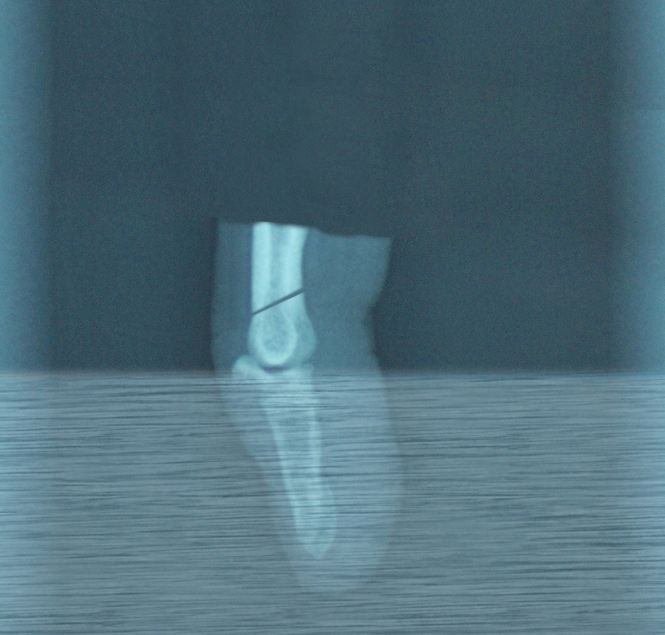
\includegraphics[width=0.5\linewidth]{images/SCP-170.jpg}
    \caption*{对象连在桌子上的手指(截断后)。骨折是由对象自己的挣扎所导致的。}
\end{figure}

\bb{试验12:}\\
\bb{试验材料:}一名D级人员,一张木桌\\
\bb{步骤:}这是第一次用活体生物对象做实验。将少量SCP-170涂在D级人员的右手食指上,然后给他“戳戳桌子”的指令。\\
\bb{结果:}对象的手指沉进桌子一个指节。虽然惊恐万状,但对象并未感到疼痛及不适,或是对接触点之下有知觉。然而,他的手指很快肿起淤紫,他的循环系统似乎一直在朝一个有去无回的区域泵血。从第一指节和第二指节间切断了手指。

\bb{试验19:}\\
\bb{试验材料:}Pratt \& Whitney F100喷射发动机一台,收容区域19b的加固屋顶\\
\bb{步骤:}SCP-170被涂在喷射发动机装备上,然后将发动机快速按进房间天花板内3.2cm(约1.25英寸)深。在连接上适当的燃料供给和控制系统之后,启动了喷射发动机。\\
\bb{结果:}摄影机监控着连接点以期观察到变形作用,期间发动机高速运转了40分钟。当连接点周围的混凝土开始出现小裂缝时,甚至在120000牛顿的力的作用下,仍未出现任何结构损坏或是两种材料分离的可能性。
